\documentclass[10pt,letterpaper]{article}
\usepackage{code/manuscript_assets/researchpreprint}
\usepackage{amsmath,amssymb,amsthm,booktabs,graphicx}
\usepackage[hidelinks]{hyperref}

\newtheorem{theorem}{Theorem}
\newtheorem{proposition}[theorem]{Proposition}
\newtheorem{corollary}[theorem]{Corollary}
\theoremstyle{definition}
\newtheorem{definition}[theorem]{Definition}

% generated by code/scripts/numbers.py -- do not edit
\newcommand{\VerGraphs}{60}
\newcommand{\VerValues}{276{,}480}
\newcommand{\VerMaxErr}{1.25\times10^{-14}}
\newcommand{\PetGap}{1.89\times10^{-15}}
\newcommand{\PetNa}{10}
\newcommand{\PetNb}{10}
\newcommand{\PetGa}{5}
\newcommand{\PetGb}{4}
\newcommand{\CycGap}{6.66\times10^{-16}}
\newcommand{\CycNa}{6}
\newcommand{\CycNb}{8}
\newcommand{\CycGa}{6}
\newcommand{\CycGb}{8}
\newcommand{\HeaGap}{7.77\times10^{-16}}
\newcommand{\HeaNa}{14}
\newcommand{\HeaNb}{14}
\newcommand{\HeaGa}{6}
\newcommand{\HeaGb}{4}
\newcommand{\XPairs}{186{,}624}
\newcommand{\XViol}{0}
\newcommand{\XSpear}{0.62}
\newcommand{\XMedRatio}{0.21}
\newcommand{\CorpusSize}{432}
\newcommand{\AnglePoints}{4{,}608}
\newcommand{\LeakPairs}{93{,}096}
\newcommand{\LeakIdentical}{3{,}843}
\newcommand{\LeakIso}{3{,}820}
\newcommand{\LeakMissed}{23}
\newcommand{\RegGThree}{560}
\newcommand{\RegCThree}{67}
\newcommand{\RegShareThree}{96.6}
\newcommand{\RegGFour}{520}
\newcommand{\RegCFour}{186}
\newcommand{\RegShareFour}{84.4}
\newcommand{\RegGFive}{520}
\newcommand{\RegCFive}{349}
\newcommand{\RegShareFive}{48.1}
\newcommand{\CenGFive}{21}
\newcommand{\CenCFive}{21}
\newcommand{\CenShareFive}{0.0}
\newcommand{\CenGSix}{112}
\newcommand{\CenCSix}{112}
\newcommand{\CenShareSix}{0.0}
\newcommand{\CenGSeven}{853}
\newcommand{\CenCSeven}{848}
\newcommand{\CenShareSeven}{1.2}
\newcommand{\CorpusLandscapes}{231}
\newcommand{\NaiveLeak}{222}
\newcommand{\NaiveLeakPct}{51}
\newcommand{\NaiveMean}{0.02599}
\newcommand{\NaiveRidge}{0.00201}
\newcommand{\NaiveSpectral}{0.00047}
\newcommand{\GroupMean}{0.02599}
\newcommand{\GroupRidge}{0.00253}
\newcommand{\GroupSpectral}{0.00551}
\newcommand{\SpecInflation}{12}
\newcommand{\RunN}{18}
\newcommand{\RunFormula}{285}
\newcommand{\RunState}{6.1}
\newcommand{\RunSpeedup}{21{,}200}
\newcommand{\GsetName}{G22}
\newcommand{\GsetN}{2{,}000}
\newcommand{\GsetM}{19{,}990}
\newcommand{\GsetT}{825}
\newcommand{\GsetSurf}{3}
\newcommand{\GsetPre}{0.07}
\newcommand{\ScalM}{1{,}199{,}424}
\newcommand{\ScalT}{155{,}845}
\newcommand{\ScalPre}{8.9}
\newcommand{\ScalSurf}{1.0}
\newcommand{\Compress}{6.0}
\newcommand{\NGset}{26}

\newcommand{\Dtv}{D_{\mathrm{TV}}}

\begin{document}

\title{A sufficient statistic for depth-one quantum approximate optimization}
\author{Molena Huynh}\email{molena.huynh@jmp.com}
\affiliation{North Carolina State University}
\maketitle

\begin{abstract}
A growing literature learns priors over quantum approximate optimization
algorithm (QAOA) angles, or transfers angles between graphs, in order to spend
fewer measurements of the quantum objective. We show that at depth one on
unweighted MaxCut this effort is unnecessary, and that its standard evaluation
protocol is unsound. From the closed form of Wang, Hadfield, Jiang and Rieffel
we prove that the depth-one landscape is a functional of a single probability
measure carrying three integers per edge: the two endpoint degrees and the
number of common neighbours. That measure is a sufficient statistic. Graphs
that share it have identical landscapes even when they are non-isomorphic, of
different order, and of different girth; we confirm this to machine precision
for the Petersen graph and the pentagonal prism. The statistic yields a
transfer guarantee that needs no quantum resources: two landscapes differ
nowhere by more than the total variation distance between their measures, and
transferring optimized angles costs at most twice that distance. We verify the
guarantee on \XPairs{} graph pairs with \XViol{} violations. Because the
measure is computable in near-linear time, exact landscapes follow for graphs
with more than a million edges, with no quantum queries, dominating every
learned prior we tested. The statistic also exposes severe degeneracy in
standard benchmarks: \RegShareThree\% of random cubic graphs share a landscape
with another sample, and a random train--test split leaves \NaiveLeakPct\% of
test graphs with an exact landscape duplicate in training, inflating the
apparent accuracy of a singular-value prior by an order of magnitude.
\end{abstract}

\section{Introduction}

The quantum approximate optimization algorithm~\cite{farhi2014qaoa,
hadfield2019alternating} prepares a variational state from a cost operator and
a mixing operator and is tuned by measuring its objective on a quantum device.
Each measured angle pair costs samples, and at shallow depth the number of
angle pairs needed to locate a good setting dominates the experimental budget.
This has motivated a substantial effort to guess good angles in advance: to
transfer optimized angles between graphs~\cite{galda2021transfer,
shaydulin2023transfer}, to exploit the observation that the objective
concentrates over instance ensembles~\cite{brandao2018fixed}, and to learn
priors that rank angle grids before any target measurement is taken. The value
of such methods is measured in queries saved.

At depth one on unweighted MaxCut, the objective has a closed form in local
graph data. Wang, Hadfield, Jiang and Rieffel~\cite{wang2018fermionic} showed
that each edge contributes a term determined by the degrees of its endpoints
and the number of vertices adjacent to both. The identity is established, and
we claim no part of it. What has not been drawn out, and what this paper is
about, is its statistical structure.

Written as a sum over edges, the identity says that the whole landscape is an
average of one fixed function over the edges of the graph. Only the
\emph{distribution} of edge data enters, not which edge carries which value,
and not any other property of the graph. The depth-one landscape is therefore a
functional of a probability measure on three non-negative integers. We call
that measure the edge statistic and show it is sufficient in the precise sense
that it determines the landscape exactly.

Four consequences follow, and they are the substance of this work. First, the
statistic is a strictly coarser invariant than isomorphism, so graphs with no
structural resemblance can have numerically identical landscapes. Second,
because the landscape is an expectation of a function bounded in $[0,1]$, two
landscapes are separated nowhere by more than the total variation distance
between their statistics; this converts parameter transfer from an empirical
practice into a certified one, computable classically in near-linear time.
Third, the standard benchmark families of the QAOA literature are severely
degenerate under this statistic, so a suite of random regular graphs contains
far fewer distinct depth-one landscapes than it contains graphs. Fourth, since
the statistic is cheap, the exact landscape is free, and no learned prior can
beat zero queries; worse, the random train--test splits used to validate such
priors place exact landscape duplicates on both sides and inflate their
reported accuracy.

We report each of these with independent numerical verification, and we state
plainly what the result does not cover. Everything here is depth one, unweighted
and noiseless. Depth two and above, weighted objectives, and hardware sampling
are outside the scope of the argument, and we do not extrapolate to them.

\section{Results}

\subsection{The landscape is a functional of an edge statistic}

For an unweighted graph $G=(V,E)$ with $n=|V|$ and $m=|E|$, write
$C=\sum_{(u,v)\in E}(I-Z_uZ_v)/2$ and $B=\sum_{v\in V}X_v$, and let
\begin{equation}
 F_G(\gamma,\beta)=\tfrac1m\,
 \langle+|\,e^{i\gamma C}e^{i\beta B}\,C\,e^{-i\beta B}e^{-i\gamma C}\,|+\rangle
 \label{eq:objective}
\end{equation}
be the normalized depth-one objective, with $|+\rangle$ the uniform product
state. For an edge $(u,v)$ define the triple
\begin{equation}
 \tau(u,v)=\bigl(\deg u-1,\ \deg v-1,\ |N(u)\cap N(v)|\bigr)
 \label{eq:triple}
\end{equation}
and let $\mu_G$ be the empirical distribution of $\tau$ over the $m$ edges, a
probability measure on $\mathbb{Z}_{\ge0}^3$. We call $\mu_G$ the \emph{edge
statistic}. Proposition~\ref{prop:whjr} in the Methods restates the identity
of Ref.~\cite{wang2018fermionic}: the contribution of edge $(u,v)$ is a fixed
function $f(\tau(u,v);\gamma,\beta)$ of its triple alone. Summing and dividing
by $m$ gives the following.

\begin{theorem}[Sufficiency]
\label{thm:sufficient}
For every graph $G$ and every angle pair,
\begin{equation}
 F_G(\gamma,\beta)=\mathbb{E}_{\tau\sim\mu_G}\bigl[f(\tau;\gamma,\beta)\bigr].
 \label{eq:sufficient}
\end{equation}
Consequently $\mu_G=\mu_H$ implies $F_G\equiv F_H$, whether or not $G$ and $H$
are isomorphic and whether or not they have the same number of vertices.
\end{theorem}

Equation~\eqref{eq:sufficient} is an immediate consequence of the identity of
Ref.~\cite{wang2018fermionic}, and we present it as such. Its content is the
converse reading: everything the depth-one landscape can express about a graph
is already contained in three integers per edge, discarded down to their
distribution.

\begin{figure}[t]
\centering
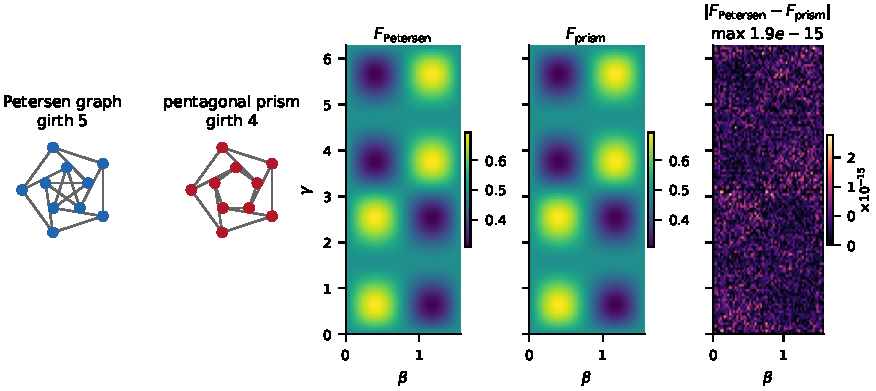
\includegraphics[width=\textwidth]{code/results_full/figures/fig1_sufficient_statistic.pdf}
\caption{\textbf{Two graphs with nothing in common have the same depth-one
landscape.} The Petersen graph and the pentagonal prism are non-isomorphic and
have different girth (\PetGa{} and \PetGb), but identical edge statistics. Their
landscapes, each computed by an independent statevector simulation rather than
by the formula, agree everywhere to $\PetGap$, which is roundoff. The right
panel shows the difference on a scale of $10^{-15}$.}
\label{fig:sufficient}
\end{figure}

\subsection{Landscape collisions between unrelated graphs}

Theorem~\ref{thm:sufficient} predicts exact collisions, and they occur among
familiar graphs. The Petersen graph and the pentagonal prism are both cubic on
ten vertices, are not isomorphic, and have girth \PetGa{} and \PetGb{}
respectively; every edge of each has triple $(2,2,0)$, so their statistics
coincide. Figure~\ref{fig:sufficient} shows their landscapes computed by two
independent statevector simulations, which agree to $\PetGap$. The Heawood
graph and the seven-prism collide in the same way, to $\HeaGap$. Collisions
also cross graph sizes: the \CycNa-cycle and the \CycNb-cycle have identical
landscapes to $\CycGap$, since both consist entirely of triples $(1,1,0)$.

Collisions are not generic. Exhaustive enumeration of connected graphs finds
none on five or six vertices, and only \CenShareSeven\% of the \CenGSeven{} connected
graphs on seven vertices share a landscape with another graph of that order.
The picture changes completely on structured families, which is where the
consequence bites.

\subsection{A transfer guarantee that needs no quantum resources}

Because $C_{uv}=(I-Z_uZ_v)/2$ is a projector, $f$ takes values in $[0,1]$, and
Eq.~\eqref{eq:sufficient} is an expectation of a bounded function. Comparing
two graphs then reduces to comparing two measures.

\begin{theorem}[Certified transfer]
\label{thm:transfer}
For all graphs $G,H$ and all angle pairs $\theta$,
\begin{equation}
 |F_G(\theta)-F_H(\theta)|\ \le\ \Dtv(\mu_G,\mu_H).
 \label{eq:supbound}
\end{equation}
If moreover $\theta^*_G$ and $\theta^*_H$ maximize $F_G$ and $F_H$ over a
common set of angles, then transferring the angles optimized on $G$ to $H$
costs
\begin{equation}
 F_H(\theta^*_H)-F_H(\theta^*_G)\ \le\ 2\,\Dtv(\mu_G,\mu_H).
 \label{eq:transferbound}
\end{equation}
\end{theorem}

Both bounds are uniform in the angles and involve no quantum quantity. The
right-hand side is a distance between two histograms of integer triples,
computable from the two graphs alone in near-linear time. Parameter transfer at
depth one therefore comes with an a priori certificate: before running
anything, one can bound exactly how much is lost by reusing another graph's
angles.

We tested the bounds on a corpus of \CorpusSize{} graphs comprising breadth-first
neighbourhoods of unweighted Stanford Gset instances~\cite{gset} together with
\mbox{Erd\H{o}s--R\'enyi}, random regular and Barab\'asi--Albert samples, giving
\XPairs{} ordered pairs. Landscapes were evaluated at \AnglePoints{} angle
points. Figure~\ref{fig:transfer} plots the realized landscape separation and
the realized transfer loss against their certificates. There are \XViol{}
violations. The bounds are valid but not tight: the median ratio of realized
separation to certificate is \XMedRatio, and the rank correlation between them
is \XSpear.

\begin{figure}[t]
\centering
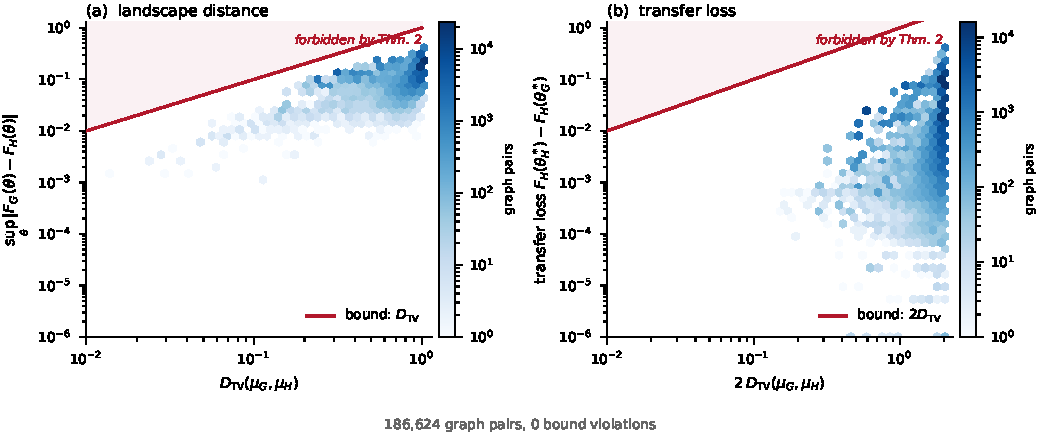
\includegraphics[width=\textwidth]{code/results_full/figures/fig2_transfer_bound.pdf}
\caption{\textbf{The transfer certificate holds everywhere.} Density of
\XPairs{} graph pairs. \textbf{a}, Realized landscape separation against the
total variation distance between edge statistics, with the bound of
Eq.~\eqref{eq:supbound}. \textbf{b}, Realized loss from transferring optimized
angles, against the bound of Eq.~\eqref{eq:transferbound}. The shaded region is
excluded by Theorem~\ref{thm:transfer}; no pair enters it.}
\label{fig:transfer}
\end{figure}

\subsection{Standard benchmark families are degenerate}

Random regular graphs are the default benchmark of the QAOA
literature~\cite{zhou2020qaoa,wurtz2021guarantees}. They are also, at depth
one, close to a single instance. Every triangle-free cubic graph has all edges
of type $(2,2,0)$ and therefore exactly one landscape, whatever its size or
structure. Sampling \RegGThree{} random cubic graphs on up to thirty vertices
yields only \RegCThree{} distinct depth-one landscapes, and \RegShareThree\% of the
sample shares a landscape with another member. Higher degree helps but does not
resolve the problem: \RegGFour{} random quartic graphs give \RegCFour{} landscapes
with \RegShareFour\% sharing, and \RegGFive{} random quintic graphs give \RegCFive{}
landscapes with \RegShareFive\% sharing (Fig.~\ref{fig:degeneracy}).

This is a statement about the benchmark, not about the algorithm. A study that
reports depth-one performance averaged over a random regular ensemble is
averaging over far fewer distinct problems than it appears to be, and its error
bars do not carry the independence they assume.

\begin{figure}[t]
\centering
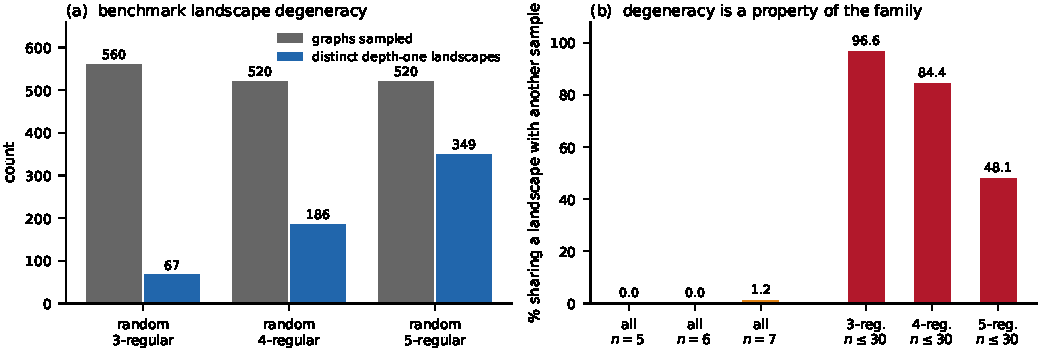
\includegraphics[width=\textwidth]{code/results_full/figures/fig3_degeneracy.pdf}
\caption{\textbf{Degeneracy is a property of the graph family.} \textbf{a},
Random regular samples contain many fewer distinct depth-one landscapes than
graphs. \textbf{b}, The fraction of graphs sharing a landscape with another
sample is negligible for exhaustively enumerated small graphs but dominant for
the regular families used as QAOA benchmarks.}
\label{fig:degeneracy}
\end{figure}

\subsection{Zero queries dominate, and random splits are leaky}

Since $\mu_G$ is computable classically, so is the entire depth-one landscape,
and the number of quantum objective queries needed to find the best angle on
any finite grid is zero. Any method that spends a positive budget is therefore
dominated at depth one. We confirm this against three predictors trained on the
corpus: the mean training landscape, ridge regression on graph features, and a
ridge prior on the singular values of the adjacency matrix. Each ranks the
angle grid, the target objective is queried in ranked order, and we report
normalized regret after $b$ queries. The exact landscape has zero regret at
$b=0$ by construction.

The more consequential finding concerns how such predictors are validated. Our
corpus of \CorpusSize{} graphs contains only \CorpusLandscapes{} distinct
landscapes, so a split that randomizes over graphs does not randomize over
problems. Under a uniform random split, \NaiveLeak{} of \CorpusSize{} test
graphs, or \NaiveLeakPct\%, have a graph with a numerically identical landscape
in their training set. Grouping the split by landscape instead removes the
duplication, and the reported accuracies change qualitatively
(Fig.~\ref{fig:regret}). At one query the singular-value prior attains regret
\NaiveSpectral{} under the random split and \GroupSpectral{} under the grouped
split, an inflation of roughly \SpecInflation-fold. Under the random split it
appears to be the best learned method, beating ridge at \NaiveRidge; under the
grouped split it is the worst, behind ridge at \GroupRidge. The training mean,
which cannot exploit duplication because it ignores the input graph, is
unchanged at \NaiveMean.

The apparent advantage of the singular-value prior is therefore an artifact of
landscape duplication, not evidence of learned structure. This is the classical
signature of leakage, and it is invisible to an audit based on graph
isomorphism: across the \LeakPairs{} corpus pairs, \LeakIdentical{} share a
landscape exactly, of which \LeakIso{} are isomorphic and \LeakMissed{} are not.
An isomorphism-grouped protocol catches most but not all of the duplication;
only grouping by the statistic itself removes it.

\begin{figure}[t]
\centering
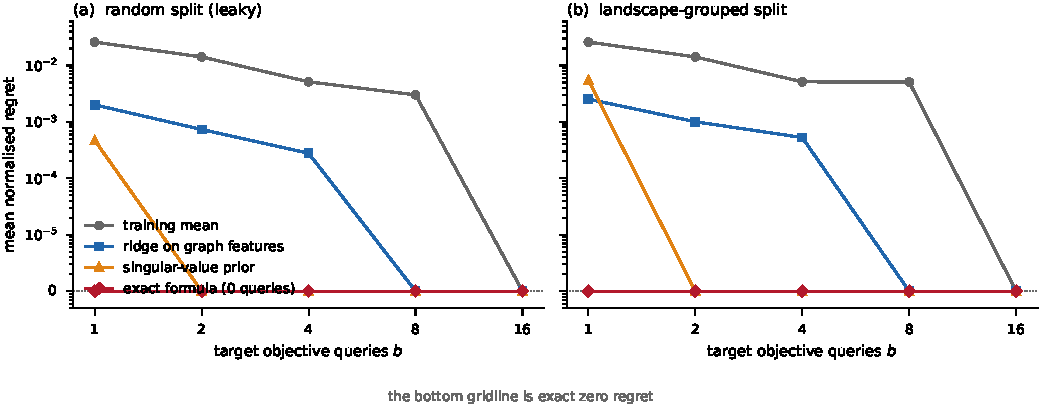
\includegraphics[width=\textwidth]{code/results_full/figures/fig4_regret.pdf}
\caption{\textbf{Learned angle priors are dominated, and their measured
accuracy depends on the split.} Mean normalized regret against the number of
target objective queries. \textbf{a}, A uniform random split over graphs, in
which \NaiveLeakPct\% of test graphs have an exact landscape duplicate in
training. \textbf{b}, A split grouped by landscape. The singular-value prior is
the best learned method in \textbf{a} and the worst in \textbf{b}. The exact
landscape uses no queries and has identically zero regret in both.}
\label{fig:regret}
\end{figure}

\subsection{Exact landscapes at scale}

Computing $\mu_G$ requires one pass for degrees and, per edge, an intersection
of the smaller endpoint neighbourhood, giving
$O(n+m+\sum_{(u,v)\in E}\min\{\deg u,\deg v\})$ preprocessing in $O(n+m)$
space. Evaluation then depends only on the number $T$ of distinct triples,
which is far smaller than $m$ on real graphs; across every graph we timed, the
median ratio $m/T$ is \Compress. On the largest unweighted Gset
instance, \GsetName{} with $n=\GsetN$ and $m=\GsetM$, the statistic has only
\GsetT{} distinct triples, takes \GsetPre~s to build, and yields an exact
81-point landscape in \GsetSurf~ms. The method reaches well past benchmark
sizes: at $m=\ScalM$ edges preprocessing takes \ScalPre~s and the landscape
\ScalSurf~s (Fig.~\ref{fig:runtime}).

The contrast with simulation is not close. At $n=\RunN$ vertices an 81-point
landscape costs \RunState~s by statevector and \RunFormula~$\mu$s from the
statistic, a factor of about \RunSpeedup. The statevector cost grows as $2^n$
and the statistic cost does not grow with $n$ at fixed $m$.

\begin{figure}[t]
\centering
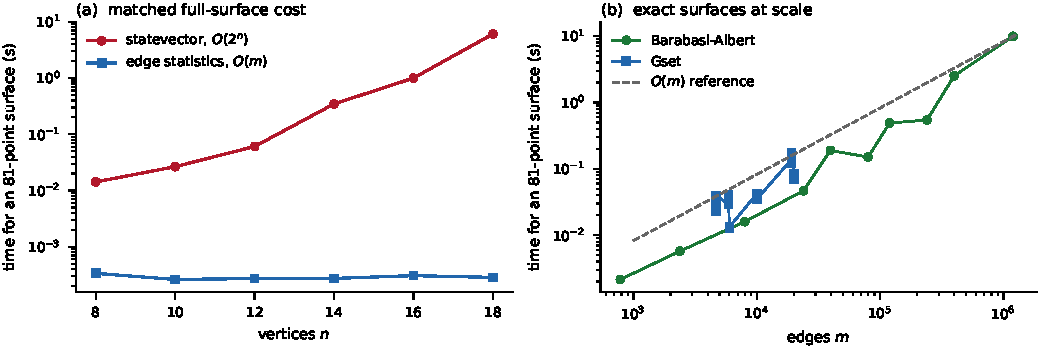
\includegraphics[width=\textwidth]{code/results_full/figures/fig5_runtime.pdf}
\caption{\textbf{Exact depth-one landscapes are cheap.} \textbf{a}, Time for an
81-point landscape by statevector simulation and from the edge statistic, on
cubic graphs. \textbf{b}, The same computation on Gset instances and on
Barab\'asi--Albert graphs up to \ScalM{} edges, against an $O(m)$ reference.}
\label{fig:runtime}
\end{figure}

\section{Discussion}

The depth-one MaxCut landscape carries three integers per edge and nothing
else. Once that is stated, the depth-one parameter transfer problem is solved
rather than approximated: the landscape is free to compute, so there is nothing
to transfer, and if one transfers anyway the loss is bounded in advance by a
histogram distance. We verified that bound on \XPairs{} graph pairs without a
violation.

The negative implications for evaluation are the part we expect to matter most.
Benchmark suites built from random regular graphs contain far fewer distinct
depth-one problems than graphs, and random train--test splits over such suites
place exact duplicates on both sides. In our corpus this inflated the measured
accuracy of a singular-value prior by an order of magnitude and reversed its
ranking against a plain ridge baseline. Any depth-one study that reports a
learned or transferred angle advantage should group its splits by the edge
statistic and should compare against the exact landscape rather than against
another learned method. Grouping by isomorphism is a partial remedy that misses
genuine collisions, and grouping by graph identity is no remedy at all.

The scope is narrow and we do not stretch it. Everything above is depth one,
unweighted and noiseless. The sufficient statistic is a property of the
depth-one light cone, and at depth two the analogous object involves larger
neighbourhoods and is not three-dimensional; whether a useful statistic of
bounded dimension survives at $p\ge2$, where closed forms are known only in
restricted settings~\cite{wurtz2021guarantees}, is open and is the natural next
question. Weighted objectives change $f$ but not the shape of the argument, and
we expect an analogous statistic on weighted triples, which we have not
verified. Sampling noise and hardware error are not modelled here at all, and a
finite-shot experiment does not inherit these guarantees. Finally, the fact
that depth one is classically solved says nothing about the value of QAOA at
depth where it is not; it says that depth one should no longer be used as
evidence for query-efficiency claims.

\section{Methods}

\subsection{The depth-one edge identity}

\begin{proposition}[Wang, Hadfield, Jiang and Rieffel~\cite{wang2018fermionic}]
\label{prop:whjr}
Let $\tau=(d_u,d_v,\lambda)$ be the triple of Eq.~\eqref{eq:triple} for an edge
$(u,v)$. Then the depth-one expectation of $C_{uv}=(I-Z_uZ_v)/2$ is
$f(\tau;\gamma,\beta)$, where
\begin{align}
 f={}&\tfrac12+\tfrac14\sin(4\beta)\sin\gamma
 \bigl(\cos^{d_u}\!\gamma+\cos^{d_v}\!\gamma\bigr)\nonumber\\
 &-\tfrac14\sin^2(2\beta)\cos^{\,d_u+d_v-2\lambda}\!\gamma
 \bigl[1-\cos^{\lambda}(2\gamma)\bigr]. \label{eq:formula}
\end{align}
\end{proposition}

The derivation is that of Ref.~\cite{wang2018fermionic} and we reproduce only
its outline to fix notation. Conjugating by the mixer gives
$e^{i\beta B}Z_uZ_ve^{-i\beta B}=c^2Z_uZ_v+cs(Z_uY_v+Y_uZ_v)+s^2Y_uY_v$ with
$c=\cos(2\beta)$ and $s=\sin(2\beta)$. Cost terms outside the closed
neighbourhood of $(u,v)$ commute through and cancel. Conjugating the remaining
Pauli strings by $e^{i\gamma C}$ and using $\langle+|P|+\rangle=0$ unless
$P\in\{I,X\}^{\otimes n}$ leaves two endpoint contributions and one
common-neighbour contribution, which are the three terms of
Eq.~\eqref{eq:formula}.

\subsection{Proof of Theorem~\ref{thm:sufficient}}

By Proposition~\ref{prop:whjr} and linearity of the expectation in
Eq.~\eqref{eq:objective},
$F_G=\frac1m\sum_{(u,v)\in E}f(\tau(u,v);\gamma,\beta)$, which is the average of
$f$ against the empirical distribution $\mu_G$ of the triples. Two graphs with
the same $\mu_G$ therefore have the same $F$ at every angle pair. Neither $n$
nor the identity of any edge appears. \qed

\subsection{Proof of Theorem~\ref{thm:transfer}}

$C_{uv}$ is a projector, so its expectation in any state lies in $[0,1]$ and
$f$ has oscillation $\operatorname{osc}f=\sup f-\inf f\le1$. Let $c$ be the
midpoint of the range of $f$. Since $\mu_G$ and $\mu_H$ are probability
measures, $\sum_\tau(\mu_G-\mu_H)(\tau)=0$, and therefore
\begin{equation}
 |F_G(\theta)-F_H(\theta)|
 =\Bigl|\sum_\tau(\mu_G-\mu_H)(\tau)\bigl(f(\tau;\theta)-c\bigr)\Bigr|
 \le\tfrac{\operatorname{osc}f}{2}\sum_\tau|(\mu_G-\mu_H)(\tau)|,
\end{equation}
which is $\operatorname{osc}f\cdot\Dtv(\mu_G,\mu_H)\le\Dtv(\mu_G,\mu_H)$ and
proves Eq.~\eqref{eq:supbound}. For Eq.~\eqref{eq:transferbound}, write
$\delta=\Dtv(\mu_G,\mu_H)$ and decompose
\begin{align}
 F_H(\theta^*_H)-F_H(\theta^*_G)
 ={}&\bigl[F_H(\theta^*_H)-F_G(\theta^*_H)\bigr]
 +\bigl[F_G(\theta^*_H)-F_G(\theta^*_G)\bigr]\nonumber\\
 &+\bigl[F_G(\theta^*_G)-F_H(\theta^*_G)\bigr].
\end{align}
The first and third brackets are at most $\delta$ by Eq.~\eqref{eq:supbound},
and the second is at most zero because $\theta^*_G$ maximizes $F_G$ over a set
containing $\theta^*_H$. \qed

\subsection{Numerical verification}

Every claim that Eq.~\eqref{eq:formula} is correct was checked against an
independent statevector simulator written for this purpose, which builds the
diagonal cost operator explicitly, applies the phase separator and the
single-qubit mixer directly, and never uses the formula. Across \VerGraphs{}
random graphs on four to fourteen vertices evaluated at \AnglePoints{} angle
points each, a total of \VerValues{} values, the maximum absolute discrepancy is
$\VerMaxErr$. The collisions of Fig.~\ref{fig:sufficient} are reported from two
statevector runs rather than from the formula, so that the agreement is not
circular.

\subsection{Corpus and protocols}

The corpus of \CorpusSize{} graphs is deterministic given fixed seeds. It
comprises ten-vertex breadth-first neighbourhoods of the first twelve
unweighted Gset instances~\cite{gset}, taken from starts $37i \bmod n$, together
with \mbox{Erd\H{o}s--R\'enyi} graphs at three densities, random regular graphs
of degree three and four, and Barab\'asi--Albert graphs, each on ten, twelve and
fourteen vertices. Of the Gset instances downloaded, \NGset{} are unweighted and
are the ones used; weighted instances are excluded because
Eq.~\eqref{eq:formula} does not apply to them.

Landscapes for the transfer study are evaluated on \AnglePoints{} angle points,
with $\gamma$ spanning its period $[0,2\pi)$ and $\beta$ spanning $[0,\pi/2)$.
The query study uses the coarser nine-by-nine grid so that a small query budget
is meaningful. Normalized regret after $b$ queries is
$r_b=\bigl(\max_\theta F-\max_{\theta\in Q_b}F\bigr)/\max_\theta F$, where
$Q_b$ holds the $b$ grid points ranked highest by the predictor. This is a
finite-grid statistic and asserts nothing about continuous global optimality.
Predictors are ridge regressions with unit regularization on standardized
features: order, size, density, the first four degree moments, triangle count
and average clustering, together with the eight largest singular values of the
adjacency matrix; the singular-value prior uses the spectral block alone.
Splits are four-fold, either uniform over graphs or over landscape classes.

\section*{Data availability}

The only external input is the Stanford Gset collection~\cite{gset}. The
package does not redistribute it; the fetch script records a SHA-256 checksum
for each instance, and the pinned value for G1 is
\texttt{73bf704d...e46d1665}. All derived results are written to
\texttt{code/results\_full/results.json}.

\section*{Code availability}

The implementation, the corpus builder, the three study scripts and the figure
generator are in \texttt{code/}. Every number in this manuscript is emitted
mechanically from \texttt{results.json} into \texttt{numbers.tex} by
\texttt{code/scripts/make\_numbers.py}; none is transcribed by hand.

\bibliographystyle{plainnat}
\bibliography{code/manuscript_assets/references}

\end{document}
